\section{Introduction}

%(1. Problem Statement & Motivation)
Learning with noisy labels (LNL) is a fundamental challenge in supervised machine learning, where errors in training data labels can significantly degrade model performance~\citep{nettleton2010study}. Deep neural networks, in particular, are prone to memorizing mislabeled examples~\citep{zhang2017understanding}, leading to overfitting and poor generalization~\citep{xie2021artificial}. Addressing this issue is crucial for real-world applications, where high-quality labeled data is expensive and human annotation errors are inevitable. Most of the research in LNL has focused on synthetic noise, where labels are artificially corrupted under controlled conditions, such as random class swaps. Although this provides a straightforward experimental setup, it fails to capture the complexity of real-world label noise~\citep{jiang2020beyond}.
\newline

%(2. Prior Work & Challenges)
A wide range of techniques have been developed to mitigate the effects of noisy labels. The problem setup shared among all of them involves training an underlying classifier (e.g., a ResNet~\citep{he2015resnet}) with a learning strategy robust to label noise. Figure~\ref{fig:overview} illustrates the general setup. Common approaches in the field include using loss functions robust to noise~\citep{ghosh2017robust, gce, wang2019symmetric}, adding specialized regularization~\citep{positive-ls, wei2021smooth}, adjusting loss based on noise estimations~\citep{forwardbackwardt, trevision, reed2014bootstrap}, filtering noisy samples~\citep{coteaching, coteaching+, jocor}, and adding additional layers to the base classifier~\citep{goldberger2017training, pes}. For a detailed survey of LNL approaches, we refer the reader to~\cite{song2022lnl}.
\newline
\begin{figure}[!ht]
    \centering
    \includegraphics[width=0.9\linewidth]{figures/lnl-drawio.pdf}
    \caption{An illustration of a setup for learning with noisy labels. During the training phase (left side), the model is trained using samples with potentially corrupted labels. The LNL algorithm tries to mitigate this noise. During the evaluation phase (right side), the trained model is evaluated with uncorrupted labels.}
    \label{fig:overview}
\end{figure}

Despite significant progress, most of these methods have been evaluated under synthetic noise assumptions, which do not fully reflect real-world annotation errors. Unlike synthetic noise, real-world noise tends to be instance-dependent~\citep{chen2021beyond}, correlating with visual similarity between classes and annotator biases~\citep{noisylabels-benchmark}. 
\newline

To bridge the gap between synthetic and real-world label noise, \citet{noisylabels-benchmark} introduced CIFAR-N, a dataset containing human-annotated label noise based on CIFAR-10 and CIFAR-100~\citep{krizhevsky2009CIFAR}. They investigate how real-world noise impacts learning and whether existing LNL methods remain effective in practical scenarios and claim that learning with real-world noise is fundamentally more challenging than with synthetic noise. Finally, they evaluate 20 state-of-the-art LNL methods on the proposed dataset.
\newline

Their key findings suggest that real-world noise differs structurally from synthetic noise, as it is feature-dependent and often reflects human annotation tendencies rather than random corruption. Additionally, deep networks memorize real-world noise more rapid-ly, overfitting human-labeled noise faster than synthetic noise, leading to different learning dynamics. Consequently, the benchmark results indicate that real-world noise poses a harder challenge for LNL methods, as models trained on synthetic noise often achieve significantly higher accuracy on clean data than those trained on human-annotated noisy labels.
\newline

Despite these contributions, the original work has several limitations. The code used to conduct the experiments is not publicly available, and key methodological details are insufficiently described, making their claims difficult to verify. Moreover, the benchmark results are published on public leaderboards and used as is in subsequent works~\citep{chen2023imprecise, xiao2023promix, zhang2025psscl}, even though flaws in the testing methodology prevent direct and fair comparisons.
To address these issues, we make the following contributions:


\begin{enumerate}
   \item We reproduce the experiments described by~\cite{noisylabels-benchmark} and open-source the code, so the experiments can be replicated by others. Our source code is publicly available at \url{https://github.com/KlemenVovk/noisy-labels}.
   \item We implement a framework to benchmark LNL methods under controlled conditions. With it, we are able to establish unified noising and testing pipelines for all methods. To our knowledge, our framework is the first such attempt in the LNL field.
   \item We benchmark LNL methods in a controlled environment, fixing the appropriate parameters and enabling a fair comparison of LNL methods on CIFAR-N.
\end{enumerate}


\section{Scope of Reproducibility} \label{sec:scope}

The original paper by~\cite{noisylabels-benchmark} introduces the CIFAR-N dataset, arguing that real-world human annotation noise differs significantly from synthetic noise and presents a more challenging learning problem. Their findings are based on a series of experiments comparing the characteristics of real and synthetic noisy labels, analyzing the memorization behavior of deep networks, and benchmarking 20, at the time, state-of-the-art LNL methods.
\newline

During their analysis of CIFAR-N, the authors make several key observations: (1) the noise distribution in CIFAR-N is imbalanced, favoring similar-looking classes, (2) misannotations primarily occur between visually similar categories, (3) the noise exhibits a mix of symmetric and asymmetric patterns, (4) some noisy labels may reflect multiple valid annotations rather than errors, and (5) learning on real-world label noise is more challenging than learning on synthetic noise. Based on these observations, they make three central claims: (i) \textbf{human annotation noise is feature-dependent}, (ii) \textbf{deep networks memorize real-world noisy labels faster than synthetic ones}, and (iii) \textbf{LNL methods more easily model synthetic noise} than real-world human annotation noise.
\newline

In this work, we aim to reproduce and validate these claims by conducting an independent evaluation of the key findings from the original study. Specifically, we investigate:
\renewcommand{\theenumi}{\roman{enumi}}%

\begin{enumerate}
    \item \textbf{Differences Between Real-World and Synthetic Noise}: We replicate the hypothesis testing methodology to quantitatively compare human annotation noise with synthetic noise. We assess whether real-world noise is 
    feature-dependent
    and whether label transitions exhibit different structural properties (Section~\ref{sec:noise-hypothesis}).
    
    \item \textbf{Memorization of Noisy Labels by Deep Networks}: We reproduce the memorization effect experiment to examine whether deep neural networks overfit real-world noisy labels faster than synthetic ones. We analyze the impact of different noise levels and label sets on memorization trends (Section~\ref{sec:noise-memorization}).
    
    \item \textbf{Benchmarking of LNL Methods}:
    We attempt to reproduce the benchmark results reported for 10 of the 20 LNL methods, evaluating their performance on both real-world and synthetic noise. We investigate inconsistencies in the reported results and assess whether the stated training methodology leads to the same outcomes (Section~\ref{sec:benchmark}).

    \item \textbf{Evaluation of Benchmarking Methodology}:
    We examine whether the benchmarking approach used in the original paper is fair and consistent across methods (Section~\ref{sec:fair-benchmark}).

\end{enumerate}

Going beyond the original study, we propose a revised benchmarking protocol that ensures comparability across different LNL techniques.
Throughout our study, we carefully document any deviations from the original methodology and highlight areas where ambiguities in the original paper may have impacted reproducibility. By open-sourcing our implementation (\url{https://github.com/KlemenVovk/noisy-labels}), we aim to provide a transparent framework for future research in learning with noisy labels.


\section{Methodology}

We follow the authors' described methodology for all experiments except when reproducing their LNL benchmark, which we justify in Section~\ref{sec:benchmark}. Where the procedures are originally not well described or are ambiguous, we describe our selected methodology in greater detail. We also present why their benchmark results should not be used as a benchmark and provide improvements that enable a fairer comparison.

\subsection{Datasets}

We use the CIFAR-N datasets provided by the benchmark authors~\cite{noisylabels-benchmark}. Their work is based on the standard CIFAR-10 and CIFAR-100 datasets~\citep{krizhevsky2009CIFAR}, consisting of $50,000$ train and $10,000$ test images with image-level class annotations. As the names suggest, CIFAR-10 includes 10 label categories, while CIFAR-100 has 100.
The authors propose noisy extensions for both datasets, which keep the original images but replace the labels with real-world noisy annotations. Only the training sets of both datasets have these, while the $10,000$ testing labels are kept from the original CIFAR-10 and -100 datasets and are considered noise-free. The $50,000$ training labels from the original CIFAR datasets are considered ground truth clean labels.
The CIFAR-10N extension includes five sets of noisy labels obtained from different annotators with varying degrees of noise.
Specifically, the authors present the following label sets:
\begin{itemize}
    \item \textbf{Random1, Random2, Random3}: These directly include the labels submitted by different annotators. These have a medium noise level, with $17.23\%$, $18.12\%$, and $17.64\%$ noise ratios, respectively.
    \item \textbf{Aggregate}: Labels in this set are obtained from Random1, Random2 and Random3 via majority voting. Whenever there is a 3-way disagreement, the label is selected randomly. Due to the aggregation, the noise level here is the lowest at $9.03\%$.
    \item \textbf{Worst}: Similarly, as in the \textit{Aggregate} set, labels here are also obtained from the three \textit{Random} sets but are aggregated so that incorrect labels are taken wherever possible. As such, the noise level here is the highest, with $40.21\%$ incorrect labels.  
\end{itemize}
Clean-to-noisy label transition matrices in Figure \ref{fig:transition-matrices} indicate percentages of misassigned labels and common mistakes (e.g., mislabeling truck as an automobile). 

\begin{figure}[!ht]
    \centering
    \includegraphics[width=0.9\textwidth]{figures/cifarn_noise_cmaps.pdf}
    \caption{\textbf{Transition matrices} of CIFAR10-N for Aggregate, Random1 and Worst label sets. A single row denotes the percentages of transitions of the row label to any of the column labels. Missing numbers indicate that no such transition was found in the provided noisy label set. The color bar is log-norm transformed to highlight noise levels.}
    \label{fig:transition-matrices}
\end{figure}

Similarly, the CIFAR-100N extension includes two sets of real-world noisy labels. Besides the original $100$ categories, the authors also present a new set of coarse annotations of $20$ super-classes to help the annotators during annotation. The annotators are first asked to assign a super-class, from which they then later select the fine-grained class. The two noisy label sets are then defined as follows:
\begin{itemize}
    \item \textbf{Coarse}: consists of the 20 super-class labels with a noise rate of $25.60\%$.
    \item \textbf{Fine}: consists of all 100 fine categories and has $40.20\%$ of noisy labels.
\end{itemize}

The authors observe that in CIFAR-100N some label noise may not necessarily indicate incorrect annotations but rather the presence of multiple valid labels within an image. We visualize some examples in Figure~\ref{fig:double-labels}. 
\newline

\begin{figure}[!ht]
    \centering
    \begin{subfigure}[b]{0.9\textwidth}
         \centering
         \includegraphics[width=\textwidth]{figures/double_labels_original.pdf}
         \caption{A reproduction of Figure 4 by~\cite{noisylabels-benchmark}.} \label{fig:2a}
     \end{subfigure}

     \begin{subfigure}[b]{0.9\textwidth}
         \centering
         \includegraphics[width=\textwidth]{figures/corrected_labels.pdf}
         \caption{Images to which their noisy labels might be better suited than their original labels.} \label{fig:2b}
     \end{subfigure}
    \caption{\textbf{Examples of training images with multiple valid labels} from CIFAR-100N. The first caption contains the clean CIFAR-100 label, and the bottom one is the human-annotated "noisy" label.}
    \label{fig:double-labels}
\end{figure}

They provide examples of such cases, with the frequent case being a fisherman holding a flatfish in his hands. We reproduce their exemplar images in Figure~\ref{fig:2a}. During our analysis, we even observed that some noisy annotations actually describe the images better than their original labels. %We show such examples in Figure~\ref{fig:2b}.







\subsection{Reproducing Noise Hypothesis Testing} \label{sec:noise-hypothesis}


\citet{noisylabels-benchmark} qualitatively and quantitatively show that real-world human noise differs from synthetic noise with hypothesis testing. We follow the same procedure while taking note of certain ambiguous decisions.
\newline

We start by fitting a ResNet-34 model on clean CIFAR-10 train labels. The authors do not explicitly explain how the model was trained, so we use the default training methodology presented in Section~\ref{sec:benchmark}.
Once trained, we use the classifier to get image embeddings for all $50,000$ training images.
\newline

Next, for each of the $N=10$ classes, we cluster its embeddings into $\nu=5$ clusters $C_{n, v}, \forall n \in N, \forall v \in \nu $ using a K-Means model.
As all cluster members belong to the same clean class, we can then obtain a $N$-dimensional transition vector for each cluster: $\mathbf{p}_{n, v} = [ \mathbb{P}(\widetilde{Y}=j | Y=n, X\in C_{n, v}) ]_{j \in [N]}$. We do this for both real-world and synthetic labels, specifically the Random1 label set and its synthetic counterpart.
We generate the synthetic label set by sampling from an asymmetric transition matrix estimated from the CIFAR-N noisy labels. Following the approach in the original paper, we compute this matrix by counting class-wise label flips between the human-annotated (noisy) labels and the clean labels. The resulting transition matrix (visualized in Figure~\ref{fig:transition-matrices}) is then used to synthesize new noisy labels, producing a synthetic counterpart following the same transition matrix but without instance-dependence.
At this point, we plot the resulting transition vectors in each class and cluster and qualitatively check for differences between the real-world and synthetic transition vectors.
\newline

We repeat the previous steps $E=10$ times, generating a new set of synthetic labels and embeddings each time. To get different embeddings, we randomly augment the images with horizontal flips and random crops.
This gives us a set of transition vectors $\{\mathbf{p}_{e,k,v}\}_{e \in [E], k \in [K], v \in [\nu]}$ for both synthetic and human noise.
From this data, we can obtain the two sets of $l_2$ distances between the transition vectors -- the human-synthetic distances:
\[
\{ d_{e,k,v}^{(1)} = || \mathbf{p}_{e,k,v}^{human} - \mathbf{p}_{e,k,v}^{synthetic} ||_2^2 \}_{e \in [E], k \in [K], v \in [\nu]}
\]
and the synthetic-synthetic distances:
\[
\{ d_{e,k,v}^{(2)} = || \mathbf{p}_{e,k,v}^{synthetic} - \mathbf{p}_{(e+1)\%E,k,v}^{synthetic} ||_2^2 \}_{e \in [E], k \in [K], v \in [\nu]}.
\]
From here on, we use the same formulation and procedures for the hypothesis test as in the original work~\cite{noisylabels-benchmark}.


\subsection{Reproducing Noise Memorization}
\label{sec:noise-memorization}

To further investigate the differences between artificial and real-world noise, ~\cite{noisylabels-benchmark}, inspect the learning behavior of a classifier trained on both sets of noisy labels. Specifically, they compare the learning behavior on \textit{Aggregate}, \textit{Random1}, and \textit{Worst} sets of real-world labels with their synthetic counterparts.
\newline

The procedure to obtain synthetic labels remains the same as described in Section \ref{sec:noise-hypothesis}.
They check whether the ratio of memorized examples increases faster for synthetic or real-world noisy labels. In a $K$-class classification task, given a classifier $f$, a feature $x$ and confidence threshold $\eta$, $x$ is memorized by $f$ if $\exists i \in [K]$ s.t. $P(f(x) = i) > \eta$.
\newline

The authors do not explain the training setup beyond the fact that ResNet-34~\citep{he2015resnet} is used as a classifier with the confidence threshold $\eta=0.95$. From the figures in the original paper, we deduce that each experiment was run for $150$ epochs. Furthermore, we assume that a smooth learning rate schedule was used, based on the shape of the memorization curves. We obtain the rest of the hyperparameters from the memorization experiments by~\cite{xie2021artificial} using the SGD optimizer without momentum and setting the initial learning rate to $\gamma=1$, weight decay to $1e-4$ and a smooth version of their learning rate scheduler ($\gamma_{t} = \gamma \cdot0.1^{\frac{t}{50}}$).

\subsection{Reproducing the Benchmark} \label{sec:benchmark}

%We integrate 10 methods for learning with noisy labels into a unified framework.
%Based on the original implementations, we include the following methods:
%\textit{Forward/Backward-T}~\citep{forwardbackwardt},
%\textit{GCE}~\citep{gce},
%\textit{Co-teaching (+)}~\citep{coteaching, coteaching+},
%\textit{T-revision}~\citep{trevision},
%\textit{Peer loss}~\citep{peerloss},
%\textit{ELR (+)}~\citep{elr},
%\textit{Divide-Mix}~\citep{dividemix},
%\textit{JoCoR}~\citep{jocor},
%\textit{Cores$^2$}~\citep{cores},
%\textit{VolMinNet}~\citep{volminnet},
%\textit{CAL}~\citep{cal},
%\textit{PES (semi)}~\citep{pes},
%\textit{SOP (+)}~\citep{sop},
%\textit{Positive-LS}~\citep{positive-ls} and
%\textit{F-divergence}~\citep{f-divergence}
%where (+) denotes that both the \textit{method} and \textit{method}+ versions %are included.
Due to the large computation cost (see Appendix~\ref{appsec:computational-requirements}), we select a subset of 10 methods that show good performance in the original results:
\textit{CE} (baseline),
\textit{Co-Teaching}~\citep{coteaching},
\textit{Co-Teaching+}~\citep{coteaching+},
\textit{ELR, ELR+}~\citep{elr},
\textit{Divide-Mix}~\citep{dividemix},
\textit{VolMinNet}~\citep{volminnet},
\textit{CAL}~\citep{cal},
\textit{PES (semi)}~\citep{pes},
\textit{SOP}, and 
\textit{SOP+}~\citep{sop}.
Here, we note that the author's reported performance for the SOP method is most likely SOP+, so we include both methods in our benchmark.
\newline

The authors do not describe the evaluation procedure for the benchmark, but we have reproduced it based on GitHub issues and personal correspondence. During training with each LNL method, the classifier is evaluated in terms of micro-averaged accuracy on a clean test set every epoch. At the end, the highest achieved accuracy is reported. Each run is repeated three times to obtain the mean accuracy and the standard deviation.
\newline

While being a crucial part of many learning strategies, the benchmark authors do not discuss the hyperparameters for each method in full detail. Therefore, we reference their official implementations as a starting point and, as described by the authors, fix the following\footnote{See \cite{noisylabels-benchmark} Appendix E.3.}:
training time to 100 epochs, a stochastic gradient descent optimizer with momentum ($0.9$), weight decay ($5e-4$), an initial learning rate of $0.1$ which decreases to $0.01$ at the 60th epoch, and a minibatch size of 128.
The authors also note that the ELR (+) and DivideMix methods received special treatment and were run using their original configurations. We observe that for SOP the pre-activation ResNet-18 was used\footnote{See  \cite{noisylabels-benchmark} caption of Table 2 .},  and based on the authors' discussion with reviewers, that the low noise configuration ($\lambda_u=0$) was used for DivideMix\footnote{See \url{https://openreview.net/forum?id=TBWA6PLJZQm} discussion with reviewer \textit{EZud}.}.
Following these findings, we use ResNet-34 for most of the learning strategies and a pre-activation ResNet-18 for SOP, ELR+, and DivideMix, consistent with the described setup.
\newline

As we later show in Section \ref{sec:results-benchmark}, following the methodology inferred from the original study, we do not reach the same results. We argue that fixing the learning rate, optimizer, and the number of epochs without redoing the hyperparameter search reduces the performance of methods (in a possibly uneven way). Instead, when using the original hyperparameter configurations for each LNL method along with the optimizers, learning rates, and training durations, most of the methods perform close to the original reported accuracy.
\newline

Given these findings, it is likely that the original authors followed a methodology closer to our reverse-engineered approach rather than the one explicitly described in their paper. However, due to inconsistencies between the paper and the available implementation, as well as the discontinued correspondence with the original authors (see Appendix~\ref{appsec:communication}), we are unable to verify this assumption with certainty.

\subsection{Making the Benchmark Fair}
\label{sec:fair-benchmark}

We argue that this approach is flawed in several aspects and present a better evaluation procedure. When benchmarking LNL methods, the authors use a clean test set to measure accuracy every epoch, selecting the highest one at the end. This overestimates the real-world performance and is thus unreliable in practice~\citep{cawley2010over}.
\newline

During our experiments, we observed that the underlying classifier strongly influences the final performance. Given that the authors do not use the same ResNet model for all LNL methods (e.g., special treatment of DivideMix, ELR, and SOP), one cannot directly compare the entries on the benchmark. This is an issue as their results are currently published on a public leaderboard\footnote{\url{https://web.archive.org/web/20250405111513/https://paperswithcode.com/task/learning-with-noisy-labels}}, making users unfamiliar with the testing methodology believe that the results are directly comparable between the entries. 
To ensure a fair comparison with state-of-the-art methods we also include two newer methods: ProMix\citep{xiao2023promix} and DISC \citep{li2023disc}.
\newline

To address these flaws, we adapt the benchmarking procedure as follows. We use the official hyperparameters for each LNL method and fix only the underlying classifier. We use the PyTorch implementation of ResNet-34 with random weight initialization. Instead of testing every epoch, we use $5\%$ of the noisy training data as a validation set to compute accuracy. We report the accuracy on the clean test set corresponding to the checkpoint with the highest validation accuracy. We present our argument on why accuracy on noisy data is a good metric for model selection in Appendix \ref{appsec:accuracy}. We repeat each run three times and report the average accuracy along with the standard deviation.


\subsection{Experimental Setup and Code} \label{sec:exp-setup-and-code}

We implement our framework using PyTorch\footnote{\url{https://pytorch.org}} and Lightning~\citep{Falcon_PyTorch_Lightning_2019}
% \footnote{\url{https://lightning.ai/docs/pytorch/stable/}} 
for easier reproducibility, distributed training, and robust, identical testing of all methods. The modularity of the framework enables easier implementation and comparison of future LNL methods. The code is publicly available at (\url{https://github.com/KlemenVovk/noisy-labels}).



\section{Results}

In this section, we describe the results obtained using the previously specified methodology. Each subsection corresponds to one of the reproducibility claims outlined in Section~\ref{sec:scope}.

\subsection{Reproduced Noise Hypothesis Testing}

We confirm the original claim that human-noisy labels in CIFAR-N differ from synthetic ones obtained from the same transition matrix.
We do not match the reported p-value entirely, ours being higher at $9.5\cdot10^{-28}$ versus $1.8\cdot10^{-36}$, reported by the original authors.
Qualitatively, the differences between the human and synthetic cluster transition vectors in Figure~\ref{fig:noise-hypothesis} are also not as prominent as in the original work. However, they still exhibit a similar pattern, with human noise varying more along the cluster dimension, which implies feature dependence. We attribute the differences to possibly different training regimes, since the original one is not described in full detail.

\begin{figure}[!ht]
    \centering
    \begin{subfigure}[b]{0.9\textwidth}
         \centering
         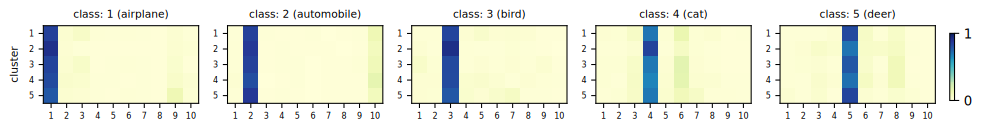
\includegraphics[width=\textwidth]{figures/human_cluster.pdf}
         \caption{Human noise (Random 1): noise level $\approx 17.23\%$.}
     \end{subfigure}
    \begin{subfigure}[b]{0.9\textwidth}
         \centering
         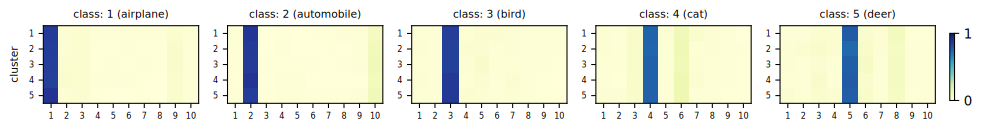
\includegraphics[width=\textwidth]{figures/synthetic_cluster.pdf}
         \caption{Synthetic class-dependent noise with the same T.}
     \end{subfigure}
    \caption{\textbf{Transition vectors} within $\nu=5$ clusters for the first $5$ classes for real-world human noise and corresponding synthetic noise. Qualitatively, human noise shows a greater diversity of transition vectors between the clusters in each class. We use the Euclidean distance for k-means clustering on $\ell^2$-normalized embeddings, which is proportional to the negative cosine similarity used by the authors.}
    \label{fig:noise-hypothesis}
\end{figure}


\subsection{Reproduced Noise Memorization} \label{sec:results-memorization}
Our reimplementation of the noise memorization experiments also supports the claims of~\cite{noisylabels-benchmark}. Figure~\ref{fig:noise-memo} presents the memorization dynamics across three label sets with increasing noise levels. The full lines lying above the dashed ones indicate that models begin memorizing real-world noisy labels more rapidly than synthetic ones. While the effect is less pronounced than in Figure 6 of ~\cite{noisylabels-benchmark}, our results consistently demonstrate that models overfit human-labeled noise faster than synthetic noise, especially under higher noise levels (\textit{Worst} label). Notably, the memorization of real-world noise remains somewhat consistent across noise levels, while synthetic labels are memorized with a higher frequency at lower noise levels. The observed discrepancies can again be attributed to differences in training configurations, as certain implementation details were either missing from the original paper or remained unclear despite our correspondence with the authors. 
We perform additional experiments using different types of synthetic noise and SGD parameters in Appendix~\ref{appsec:memorization}. While the memorization dynamics differ under different synthetic noises and hyperparameters, the observations of the original authors hold: deep neural nets memorize features more easily when learning with real-world human annotations than synthetic ones.

\begin{figure}[!ht]
    \centering
    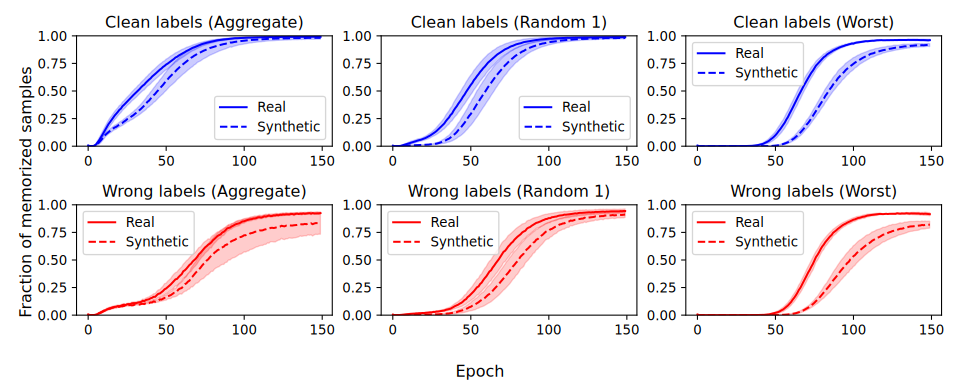
\includegraphics[width=0.9\textwidth]{figures/memorization.pdf}
    \caption{\textbf{Noise memorization effects}. The \textcolor{red}{red} line denotes the proportion of memorized (wrongly labeled) samples, and the \textcolor{blue}{blue} line denotes that of correctly annotated ones. The models start to memorize the human noisy labels (full line) faster than the synthetic ones (dashed line). }
    \label{fig:noise-memo}
\end{figure}




\subsection{Reproduced Benchmark} \label{sec:results-benchmark}

Table~\ref{tab:config-comparison} shows the results obtained using the evaluation methodology described in~\cite{noisylabels-benchmark} on the \textit{Aggregate} label set. There are significant differences between the results reported in the original paper and those obtained when following the methodology fully (fixing the same optimizer, learning rate schedule, and number of epochs for all methods). Upon further investigation, we repeat the experiments using the methods' original configurations. The results are closer to those reported by~\cite{noisylabels-benchmark}. 

\begin{table}[!ht]
    \centering
    \caption{\textbf{Comparison with the reported results on the \textit{Aggregate} label.} We report the results (accuracy$\pm$std) obtained using our reimplementation of the configuration described by the authors, the original configuration for each method, and the reported results. Only the results for which the authors use original configurations (denoted by $^*$) are close to the reported ones. 
    }
    \label{tab:config-comparison}
{
    \footnotesize
    \begin{tabular}{ccc|c}
    \toprule
    \textbf{Method} & \textbf{Described Config} & \textbf{Original Config} & \textbf{Reported} \\
    \midrule
    CE              & $91.70$\tiny{$  \pm 0.07 $}  & $91.70$\tiny{$  \pm 0.07 $}  & $87.77$\tiny{$  \pm 0.38 $} \\
    Co-teaching     & $90.25$\tiny{$  \pm 0.13 $}  & $91.93$\tiny{$  \pm 0.25 $}  & $91.20$\tiny{$  \pm 0.13 $} \\
    Co-teaching+    & $86.20$\tiny{$  \pm 0.88 $}  & $91.15$\tiny{$  \pm 0.08 $}  & $90.61$\tiny{$  \pm 0.22 $} \\
    ELR$^*$             & $93.00$\tiny{$  \pm 0.19 $}  & $93.00$\tiny{$  \pm 0.19 $}  & $92.38$\tiny{$  \pm 0.64 $} \\
    ELR+$^*$            & $95.32$\tiny{$  \pm 0.06 $}  & $95.32$\tiny{$  \pm 0.06 $}  & $94.83$\tiny{$  \pm 0.10 $} \\
    DivideMix$^*$       & $95.62$\tiny{$  \pm 0.09 $}  & $95.62$\tiny{$  \pm 0.09 $}  & $95.01$\tiny{$  \pm 0.71 $} \\
    VolMinNet       & $84.02$\tiny{$  \pm 6.61 $}  & $90.47$\tiny{$  \pm 0.17 $}  & $89.70$\tiny{$  \pm 0.21 $} \\
    CAL             & $91.76$\tiny{$  \pm 0.22 $}  & $91.84$\tiny{$  \pm 0.23 $}  & $91.97$\tiny{$  \pm 0.32 $} \\
    PES (semi)      & $91.53$\tiny{$  \pm 0.44 $}  & $94.64$\tiny{$  \pm 0.05 $}  & $94.66$\tiny{$  \pm 0.18 $} \\
    SOP+ & $93.17$\tiny{$  \pm 0.66 $}  & $96.04$\tiny{$  \pm 0.15 $}  & $95.61$\tiny{$  \pm 0.13 $} \\
    \bottomrule
    \end{tabular}
}
\end{table}

We reproduce the authors' results on the CIFAR-N dataset using the configurations specific to each evaluated method. We compare our results with those reported by \cite{noisylabels-benchmark} (Tables 2 and 8). Table \ref{tab:bechmark-results} shows the results of the reimplemented methods for all label sets in CIFAR-N.


\begin{table}[!ht]
\centering
\caption{\textbf{Results based on the original methods' configurations.} Results for most of the methods match those reported in the original work. We report the average best test set accuracy and standard deviation of three runs. }
\resizebox{\textwidth}{!}{*
    \begin{tabular}{ccccccc|cc}
\toprule
 \multirow{2}{*}{\textbf{Method}} & \multicolumn{6}{c|}{\textbf{CIFAR-10N}} & \multicolumn{2}{c}{\textbf{CIFAR-100N}} \\
 & Clean & Aggregate & Random 1 & Random 2 & Random 3 & Worst & \multicolumn{1}{c}{Clean} & \multicolumn{1}{c}{Noisy} \\
\midrule
CE & $94.21$\footnotesize{$  \pm 0.12 $} & $91.70$\footnotesize{$  \pm 0.07 $} & $90.20$\footnotesize{$  \pm 0.04 $} & $90.12$\footnotesize{$  \pm 0.13 $} & $90.08$\footnotesize{$  \pm 0.05 $} & $83.91$\footnotesize{$  \pm 0.08 $} & $76.23$\footnotesize{$  \pm 0.19 $} & $61.19$\footnotesize{$  \pm 0.51 $} \\
Co-teaching & $92.15$\footnotesize{$  \pm 0.11 $} & $91.93$\footnotesize{$  \pm 0.25 $} & $90.69$\footnotesize{$  \pm 0.07 $} & $90.51$\footnotesize{$  \pm 0.14 $} & $90.56$\footnotesize{$  \pm 0.22 $} & $80.92$\footnotesize{$  \pm 0.43 $} & $72.24$\footnotesize{$  \pm 0.44 $} & $54.48$\footnotesize{$  \pm 0.27 $} \\
Co-teaching+ & $92.90$\footnotesize{$  \pm 0.22 $} & $91.15$\footnotesize{$  \pm 0.08 $} & $89.82$\footnotesize{$  \pm 0.13 $} & $89.64$\footnotesize{$  \pm 0.19 $} & $89.77$\footnotesize{$  \pm 0.26 $} & $82.36$\footnotesize{$  \pm 0.04 $} & $70.39$\footnotesize{$  \pm 0.45 $} & $55.46$\footnotesize{$  \pm 0.34 $} \\
ELR & $93.97$\footnotesize{$  \pm 0.12 $} & $93.00$\footnotesize{$  \pm 0.19 $} & $92.20$\footnotesize{$  \pm 0.10 $} & $92.05$\footnotesize{$  \pm 0.12 $} & $92.18$\footnotesize{$  \pm 0.17 $} & $87.89$\footnotesize{$  \pm 0.14 $} & $75.64$\footnotesize{$  \pm 0.21 $} & $63.72$\footnotesize{$  \pm 0.38 $} \\
ELR+ & $95.81$\footnotesize{$  \pm 0.16 $} & $95.32$\footnotesize{$  \pm 0.06 $} & $94.89$\footnotesize{$  \pm 0.11 $} & $94.88$\footnotesize{$  \pm 0.08 $} & $94.93$\footnotesize{$  \pm 0.07 $} & $91.75$\footnotesize{$  \pm 0.06 $} & $\boldsymbol{78.82}$\footnotesize{$\pm 0.24$} & $67.87$\footnotesize{$  \pm 0.07 $} \\
DivideMix & $95.51$\footnotesize{$  \pm 0.00 $} & $95.62$\footnotesize{$  \pm 0.09 $} & $\boldsymbol{95.72}$\footnotesize{$\pm 0.11$} & $\boldsymbol{95.78}$\footnotesize{$\pm 0.10$} & $95.71$\footnotesize{$  \pm 0.09 $} & $\boldsymbol{93.10}$\footnotesize{$\pm 0.10$} & $78.22$\footnotesize{$  \pm 0.06 $} & $\boldsymbol{70.91 }$\footnotesize{$\pm 0.09$}\\
VolMinNet & $92.71$\footnotesize{$  \pm 0.02 $} & $90.47$\footnotesize{$  \pm 0.17 $} & $88.90$\footnotesize{$  \pm 0.51 $} & $88.81$\footnotesize{$  \pm 0.17 $} & $88.67$\footnotesize{$  \pm 0.10 $} & $80.87$\footnotesize{$  \pm 0.25 $} & $72.73$\footnotesize{$  \pm 0.65 $} & $58.30$\footnotesize{$  \pm 0.05 $} \\
CAL & $93.78$\footnotesize{$  \pm 0.18 $} & $91.84$\footnotesize{$  \pm 0.23 $} & $91.10$\footnotesize{$  \pm 0.26 $} & $90.60$\footnotesize{$  \pm 0.10 $} & $90.61$\footnotesize{$  \pm 0.12 $} & $84.82$\footnotesize{$  \pm 0.23 $} & $74.53$\footnotesize{$  \pm 0.21 $} & $60.13$\footnotesize{$  \pm 0.33 $} \\
PES (semi) & $94.75$\footnotesize{$  \pm 0.16 $} & $94.64$\footnotesize{$  \pm 0.05 $} & $95.20$\footnotesize{$  \pm 0.08 $} & $95.26$\footnotesize{$  \pm 0.13 $} & $95.20$\footnotesize{$  \pm 0.11 $} & $92.58$\footnotesize{$  \pm 0.05 $} & $77.77$\footnotesize{$  \pm 0.33 $} & $70.32$\footnotesize{$  \pm 0.28 $} \\
SOP+ & $\boldsymbol{96.53}$\footnotesize{$\pm 0.05$} & $\boldsymbol{96.04}$\footnotesize{$\pm 0.15$} & $95.70$\footnotesize{$  \pm 0.07 $} & $95.62$\footnotesize{$  \pm 0.18 $} & $\boldsymbol{95.75 }$\footnotesize{$\pm 0.14$} & $92.89$\footnotesize{$  \pm 0.09 $} & $77.90$\footnotesize{$  \pm 0.29 $} & $63.88$\footnotesize{$  \pm 0.32 $} \\
SOP & $93.76$\footnotesize{$  \pm 0.26 $} & $91.69$\footnotesize{$  \pm 0.76 $} & $89.83$\footnotesize{$  \pm 0.24 $} & $90.57$\footnotesize{$  \pm 0.46 $} & $90.88$\footnotesize{$  \pm 0.15 $} & $83.66$\footnotesize{$  \pm 0.64 $} & $72.97$\footnotesize{$  \pm 1.15 $} & $56.17$\footnotesize{$  \pm 1.02 $} \\
\bottomrule
\end{tabular}
}
\label{tab:bechmark-results}
\end{table}

For most of the methods, we are able to reproduce the results reported by the authors. One notable difference is that the baseline CE method performs much better in our experiments. The discrepancy between our and the reported baseline results is investigated in Appendix~\ref{appsec:ce}. 
Some methods use noise rate as an input parameter~\citep{coteaching, coteaching+, dividemix}. The parameter is fixed to the default value obtained from the original implementations. The justification for such a decision is that one does not always know how many labels are noisy in a real-world scenario. This way, the experimental protocol remains consistent, and the comparison is fair to all the methods. The decision to fix the noise level parameter could explain the difference in the Co-teaching(+) methods' performance on the CIFAR-100N noisy label set. 
Similarly, in the case of SOP(+) methods, symmetric noise type was assumed as an input parameter, which might explain the gap in performance on CIFAR-100N.


\subsubsection{Human Noise vs. Synthetic Noise}

Following the protocol described by the original authors, we rerun the experiment with synthetic noisy labels and compare the differences in accuracy for each entry. We subtract the real accuracies from the newly obtained synthetic ones and report the difference in Table~\ref{tab:synthetic-real}.

\begin{table}[!ht]
    \centering
    \caption{\textbf{ Differences between the real-world and synthetic test accuracies: $\text{acc}_{\text{syn}}-\text{acc}_{\text{real}}$}. Negative gaps representing the method performed better when training on human noise are highlighted in \textcolor{red}{red}. For CIFAR-10N, most of the methods perform better on synthetic noise, indicating a harder learning task when learning from human-assigned labels. For CIFAR-100N, this is not the case. We report the expected difference in best test set accuracy and standard deviation.}
{ \footnotesize
    \begin{tabular}{cccccc|c}
\toprule
 \multirow{2}{*}{\textbf{Method}} & \multicolumn{5}{c|}{\textbf{CIFAR-10N}} & \multicolumn{1}{c}{\textbf{CIFAR-100N}} \\
 & Aggregate & Random 1 & Random 2 & Random 3 & Worst & \multicolumn{1}{c}{Noisy} \\
\midrule
CE & $0.71$\tiny{$  \pm 0.10 $} & $0.93$\tiny{$  \pm 0.39 $} & $1.01$\tiny{$  \pm 0.26 $} & $1.10$\tiny{$  \pm 0.05 $} & $3.06$\tiny{$  \pm 0.21 $} & $1.89$\tiny{$  \pm 0.51 $} \\
Co-teaching & $0.89$\tiny{$  \pm 0.27 $} & $0.46$\tiny{$  \pm 0.08 $} & $0.09$\tiny{$  \pm 0.15 $} & $0.34$\tiny{$  \pm 0.23 $} & $1.40$\tiny{$  \pm 0.85 $} & \color{red}$-2.26$\tiny{$  \pm 0.36 $} \\
Co-teaching+ & $1.05$\tiny{$  \pm 0.16 $} & $1.24$\tiny{$  \pm 0.14 $} & $1.12$\tiny{$  \pm 0.19 $} & $1.19$\tiny{$  \pm 0.34 $} & $2.92$\tiny{$  \pm 0.31 $} & \color{red}$-1.94$\tiny{$  \pm 1.10 $} \\
ELR & $0.12$\tiny{$  \pm 0.21 $} & $0.31$\tiny{$  \pm 0.18 $} & $0.50$\tiny{$  \pm 0.13 $} & $0.31$\tiny{$  \pm 0.18 $} & \color{red}$-3.82$\tiny{$  \pm 0.91 $} & \color{red}$-0.71$\tiny{$  \pm 0.49 $} \\
ELR+ & $0.20$\tiny{$  \pm 0.08 $} & $0.31$\tiny{$  \pm 0.13 $} & $0.32$\tiny{$  \pm 0.08 $} & $0.33$\tiny{$  \pm 0.08 $} & \color{red}$-0.66$\tiny{$  \pm 2.48 $} & \color{red}$-0.28$\tiny{$  \pm 0.10 $} \\
DivideMix$^*$ & $0.56$\tiny{$  \pm 0.10 $} & $0.47$\tiny{$  \pm 0.12 $} & $0.54$\tiny{$  \pm 0.10 $} & $0.44$\tiny{$  \pm 0.11 $} & $1.94$\tiny{$  \pm 0.11 $} & $1.08$\tiny{$  \pm 0.48 $} \\
VolMinNet & $0.89$\tiny{$  \pm 0.17 $} & $1.15$\tiny{$  \pm 0.51 $} & $1.14$\tiny{$  \pm 0.18 $} & $1.41$\tiny{$  \pm 0.11 $} & $3.68$\tiny{$  \pm 0.67 $} & $3.11$\tiny{$  \pm 0.15 $} \\
CAL & \color{red}$-0.09$\tiny{$  \pm 0.37 $} & \color{red}$-0.76$\tiny{$  \pm 0.31 $} & \color{red}$-0.23$\tiny{$  \pm 0.36 $} & \color{red}$-0.25$\tiny{$  \pm 0.19 $} & \color{red}$-0.34$\tiny{$  \pm 0.23 $} & \color{red}$-0.57$\tiny{$  \pm 0.33 $} \\
PES (semi) & $0.29$\tiny{$  \pm 0.30 $} & $0.31$\tiny{$  \pm 0.10 $} & $0.41$\tiny{$  \pm 0.23 $} & $0.39$\tiny{$  \pm 0.11 $} & $1.71$\tiny{$  \pm 0.26 $} & $0.09$\tiny{$  \pm 0.77 $} \\
SOP+ & $0.25$\tiny{$  \pm 0.16 $} & $0.38$\tiny{$  \pm 0.08 $} & $0.48$\tiny{$  \pm 0.18 $} & $0.45$\tiny{$  \pm 0.15 $} & $2.07$\tiny{$  \pm 0.09 $} & $0.89$\tiny{$  \pm 0.36 $} \\
SOP & $0.70$\tiny{$  \pm 0.99 $} & $1.20$\tiny{$  \pm 0.83 $} & $0.17$\tiny{$  \pm 0.46 $} & $0.86$\tiny{$  \pm 0.29 $} & $2.73$\tiny{$  \pm 1.29 $} & $2.44$\tiny{$  \pm 1.02 $} \\
\bottomrule
\end{tabular}
}

    \label{tab:synthetic-real}
\end{table}

We can see that, for the most part, LNL methods perform better on synthetic data. This is at least the case for CIFAR-10N, while for CIFAR-100N, the results are evenly split, with $5$ methods performing better and $5$ methods performing worse. This matches observations reported in~\cite{noisylabels-benchmark}, indicating that learning on real-world noise is more difficult to handle. 

\subsection{Fair LNL Benchmark}\label{sec:our-benchmark}

We now report the performance of the methods when using our benchmark as described in Section~\ref{sec:fair-benchmark}. In our evaluation, we separate the methods that train two classifiers to make a fairer comparison. In this case, we follow the original implementations and use both models and average their final predictions when calculating the accuracies. The results are summarized in Table~\ref{tab:our-benchmark}. We report the test set accuracy on the clean test for the checkpoint that achieved the highest accuracy on the noisy validation set. A similar approach to be used in practice was suggested by~\cite{jiang2020beyond}. For details on our choice, please refer to Appendix~\ref{appsec:accuracy}. 
\newline

% CE beats: on clean(CAL, SOP, VOLMINNET), on aggre(CAL SOP VOLMINNET), on rand1(CAL SOP VOLMINNET), rand2(CAL SOP VOLMINNET)
Looking at the results in Table~\ref{tab:our-benchmark}, we first observe that all methods perform worse than in Table~\ref{tab:bechmark-results}. This is because we use the PyTorch ResNet-34 implementation here instead of the modified one used by the authors (more on that in Appendix~\ref{appsec:hyperparams}). Otherwise, the model ranking remains similar, with DivideMix~\citep{dividemix} and SOP+~\citep{sop} performing best from the methods used in the original work. The state-of-the-art method ProMix consistently outperforms all methods on CIFAR-10N. However, on CIFAR-100N, DivideMix retains the top ranking. Among the methods that use a single model, SOP+ outperforms the newer DISC method on CIFAR-10N, while the latter achieves the best performance on CIFAR-100N. We still observe that baseline CE training performs better than previously reported, consistently beating CAL~\citep{cal}, VolMinNet~\citep{volminnet}, and SOP~\citep{sop}.


\begin{table}[!ht]
    \centering
    \caption{\textbf{Fair LNL Benchmark}. To ensure a fair comparison, all methods utilize a ResNet-34 backbone and are evaluated using their original hyperparameter configurations. We report the test accuracy for the model checkpoint that achieves the highest validation accuracy on noisy labels. Since some methods train two classification models, we identify the best-performing method within each group (\underline{underlined}) and the overall best-performing method (\textbf{bolded}). The top group utilizes a single model, and the bottom group two. For all methods, we report the mean and standard deviation across three runs.
    }
    \label{tab:our-benchmark}
    \resizebox{\textwidth}{!}{*
    \begin{tabular}{ccccccc|cc}
\toprule
 \multirow{2}{*}{\textbf{Method}} & \multicolumn{6}{c|}{\textbf{CIFAR-10N}} & \multicolumn{2}{c}{\textbf{CIFAR-100N}} \\
 & Clean & Aggregate & Random 1 & Random 2 & Random 3 & Worst & \multicolumn{1}{c}{Clean} & \multicolumn{1}{c}{Noisy} \\
\midrule

CE & $85.50$\footnotesize{$  \pm 0.25 $} & $83.50$\footnotesize{$  \pm 0.23 $} & $81.96$\footnotesize{$  \pm 0.77 $} & $82.00$\footnotesize{$  \pm 0.13 $} & $82.19$\footnotesize{$  \pm 0.31 $} & $75.48$\footnotesize{$  \pm 0.30 $} & $59.18$\footnotesize{$  \pm 0.18 $} & $49.51$\footnotesize{$  \pm 0.39 $} \\
ELR+ & $88.56$\footnotesize{$  \pm 0.23 $} & $87.76$\footnotesize{$  \pm 0.16 $} & $86.75$\footnotesize{$  \pm 0.15 $} & $86.94$\footnotesize{$  \pm 0.07 $} & $86.97$\footnotesize{$  \pm 0.07 $} & $81.50$\footnotesize{$  \pm 0.12 $} & $61.80$\footnotesize{$  \pm 0.25 $} & $52.91$\footnotesize{$  \pm 0.27 $} \\
VolMinNet & $82.57$\footnotesize{$  \pm 0.20 $} & $80.42$\footnotesize{$  \pm 0.36 $} & $79.18$\footnotesize{$  \pm 0.10 $} & $78.54$\footnotesize{$  \pm 0.30 $} & $78.56$\footnotesize{$  \pm 0.13 $} & $72.07$\footnotesize{$  \pm 0.49 $} & $51.27$\footnotesize{$  \pm 0.18 $} & $42.39$\footnotesize{$  \pm 0.74 $} \\
CAL & $83.38$\footnotesize{$  \pm 0.47 $} & $81.51$\footnotesize{$  \pm 0.21 $} & $79.64$\footnotesize{$  \pm 0.45 $} & $79.50$\footnotesize{$  \pm 0.31 $} & $79.67$\footnotesize{$  \pm 0.26 $} & $73.08$\footnotesize{$  \pm 0.88 $} & $58.02$\footnotesize{$  \pm 0.17 $} & $47.37$\footnotesize{$  \pm 0.49 $} \\
PES (semi) & $87.08$\footnotesize{$  \pm 0.08 $} & $86.62$\footnotesize{$  \pm 0.23 $} & $87.63$\footnotesize{$  \pm 0.11 $} & $87.47$\footnotesize{$  \pm 0.20 $} & $86.80$\footnotesize{$  \pm 0.66 $} & $84.12$\footnotesize{$  \pm 0.34 $} & $60.51$\footnotesize{$  \pm 0.14 $} & $52.95$\footnotesize{$  \pm 0.47 $} \\
SOP & $82.12$\footnotesize{$  \pm 0.43 $} & $79.78$\footnotesize{$  \pm 0.85 $} & $79.22$\footnotesize{$  \pm 0.57 $} & $79.37$\footnotesize{$  \pm 0.29 $} & $78.66$\footnotesize{$  \pm 0.57 $} & $71.76$\footnotesize{$  \pm 1.98 $} & $52.61$\footnotesize{$  \pm 0.43 $} & $40.98$\footnotesize{$  \pm 0.28 $} \\
SOP+ & \underline{$90.09$\footnotesize{$  \pm 0.03 $}} & \underline{$89.50$\footnotesize{$  \pm 0.11 $}} & \underline{$88.82$\footnotesize{$  \pm 0.43 $}} & \underline{$88.99$\footnotesize{$  \pm 0.16 $}} & \underline{$88.72$\footnotesize{$  \pm 0.19 $}} & \underline{$85.18$\footnotesize{$  \pm 0.59 $}} & $61.27$\footnotesize{$  \pm 0.39 $} & $50.85$\footnotesize{$  \pm 0.06 $} \\
DISC & $89.12$\footnotesize{$  \pm 0.12 $} & $88.12$\footnotesize{$  \pm 0.24 $} & $87.31$\footnotesize{$  \pm 0.28 $} & $87.55$\footnotesize{$  \pm 0.25 $} & $87.44$\footnotesize{$  \pm 0.33 $} & $83.04$\footnotesize{$  \pm 0.13 $} & \underline{$62.13$\footnotesize{$  \pm 0.37 $}} & \underline{$53.09$\footnotesize{$  \pm 0.47 $}} \\

\midrule

Co-teaching & $86.56$\footnotesize{$  \pm 0.08 $} & $86.56$\footnotesize{$  \pm 0.27 $} & $85.26$\footnotesize{$  \pm 0.15 $} & $85.11$\footnotesize{$  \pm 0.27 $} & $84.56$\footnotesize{$  \pm 0.22 $} & $75.62$\footnotesize{$  \pm 0.32 $} & $57.07$\footnotesize{$  \pm 0.16 $} & $43.26$\footnotesize{$  \pm 0.43 $} \\
Co-teaching+ & $86.59$\footnotesize{$  \pm 0.12 $} & $85.16$\footnotesize{$  \pm 0.32 $} & $83.71$\footnotesize{$  \pm 0.28 $} & $84.20$\footnotesize{$  \pm 0.21 $} & $83.92$\footnotesize{$  \pm 0.15 $} & $76.71$\footnotesize{$  \pm 0.50 $} & $54.76$\footnotesize{$  \pm 0.58 $} & $44.25$\footnotesize{$  \pm 0.34 $} \\
ELR+ & $88.56$\footnotesize{$  \pm 0.23 $} & $87.76$\footnotesize{$  \pm 0.16 $} & $86.75$\footnotesize{$  \pm 0.15 $} & $86.94$\footnotesize{$  \pm 0.07 $} & $86.97$\footnotesize{$  \pm 0.07 $} & $81.50$\footnotesize{$  \pm 0.12 $} & $61.80$\footnotesize{$  \pm 0.25 $} & $52.91$\footnotesize{$  \pm 0.27 $} \\
DivideMix & $89.59$\footnotesize{$  \pm 0.12 $} & $89.36$\footnotesize{$  \pm 0.22 $} & $89.34$\footnotesize{$  \pm 0.10 $} & $89.61$\footnotesize{$  \pm 0.10 $} & $89.28$\footnotesize{$  \pm 0.31 $} & $86.82$\footnotesize{$  \pm 0.17 $} & \underline{$\boldsymbol{64.21}$\footnotesize{$\pm 0.02$}} & \underline{$\boldsymbol{56.21}$\footnotesize{$\pm 0.38$}} \\
ProMix & \underline{$\boldsymbol{91.53}$\footnotesize{$\pm 0.26$}} & \underline{$\boldsymbol{90.72}$\footnotesize{$ \pm 0.14$}} & \underline{$\boldsymbol{90.57 }$\footnotesize{$\pm 0.20$}} & \underline{$\boldsymbol{90.61 }$\footnotesize{$\pm 0.13$}} & \underline{$\boldsymbol{90.61 }$\footnotesize{$\pm 0.25$}} & \underline{$\boldsymbol{88.99}$\footnotesize{$ \pm 0.14$}} & $63.53$\footnotesize{$  \pm 0.03 $} & $55.67$\footnotesize{$  \pm 0.10 $} \\
\bottomrule
\end{tabular}
}
\end{table}

\section{Discussion}

We managed to reproduce the hypothesis testing and noise memorization effects. Due to a partially unclear description of the experiment protocol, we do not obtain the same results as the authors, but the results nevertheless lead to the same conclusions. The real-world label noise is indeed different from its synthetic counterpart, and the classifiers start to overfit on it faster, which indicates a harder learning task.

While the authors describe the benchmarking experiment in some detail, we fail to reach the same results using their methodology. Instead, when we use the original hyperparameter configurations for each LNL method, we obtain results closer to the reported accuracy for most of the methods. Perhaps most interesting is that the baseline cross-entropy training performs significantly better than expected, outperforming several methods designed explicitly for LNL scenarios even in the most difficult noise settings. This behavior also persists outside our framework, even in the original code provided by the authors, as we show in Appendix \ref{appsec:ce}. This finding leaves an avenue for possible future work. We provide additional comments on reproducibility and our correspondence with the authors in Appendix~\ref{appsec:reproducibility}. 



\subsection{Additional Observations} \label{sec:additional-observations}

During our implementation of several LNL methods, we noticed that the original implementations incorrectly generate synthetic noise. This raises the question of their reported performances.
The symmetric noise produced by the official DivideMix~\citep{dividemix} implementation\footnote{\url{https://github.com/LiJunnan1992/DivideMix/blob/39740b267147466bac0779de91d969909ab3b65f/dataloader_cifar.py\#L58-L74}} uses a biased noise rate. For a given noise rate $r$, their implementation randomly selects a fraction $r$ of clean labels. The noisy labels are sampled uniformly from all classes $k$. This results in $\frac{1}{k}$ of the samples agreeing with the original label, resulting in the actual noise rate being $\widetilde{r} = r - \frac{1}{k} r$ instead of $r$. This is especially evident in high-noise scenarios where DivideMix performs best.
We observe an even bigger error in the ELR~\citep{elr} implementation of synthetic noise. The method uses two models trained on separate datasets, which are both noised independently, while also producing noisy labels with a decreased noise rate $\widetilde{r}$\footnote{\url{https://github.com/shengliu66/ELR/blob/909687a4621b742cb5b8b44872d5bc6fce38bdd3/ELR/data_loader/cifar10.py\#L73-L80}} described above. 
Here,  without loss of generality, we treat the sample as noisy and as having the wrong label in the first dataset.
This results in the probability of at least one of the models observing the correct label for a sample given that the sample is noisy, being $1 - \widetilde{r}$ instead of 0. 
\newline

This brings into question the results reported in the respective original works. However, for our benchmark reproduction, where human noise is used and synthetic noise pipelines are unified, the results are unaffected, and both methods rank among the top-performing ones.

\subsection{Conclusion} 

This reproducibility study examined the claims made by ~\cite{noisylabels-benchmark} regarding real-world label noise. We successfully replicated the original noise structure hypothesis testing and noise memorization experiments with minor quantitative discrepancies likely stemming from undisclosed training details. Despite these discrepancies, our results support the authors' claim that learning on datasets with real-world noisy labels is more challenging than with synthetic noise. However, our attempts to reproduce the benchmark results revealed significant deviations. Through a detailed review and reverse engineering of the original codebase, we identified inconsistencies in the paper’s description, particularly regarding hyperparameter configurations. We then developed a unified framework for LNL methods, accompanied by an improved benchmarking procedure, incorporating a validation set on noisy data and consistent use of the ResNet-34 architecture. This framework provides a more robust platform for evaluating LNL methods, especially in scenarios where clean validation data is unavailable. Our findings highlight the need for comprehensive documentation and transparency in scientific research to ensure reproducibility and foster progress in the field.

